%		
		\subsection{Collisions and Reactions}\label{sec:negiondynamics}
%	
			\paragraph{Elastic Scattering}%
			The elastic collisions of $(1)$--$(3)$ conserve the particle numbers. Those are inter-species scattering processes, which will be assumed to have an isotropic inincident angle dependency~\cite{Bronold07b}. Intra-species elastic collisions were not very important at the selected parameter regions, though ion-ion scattering can strongly incluence the IEDF structure of the concerned densities are very high. However, for the electron species a binary \emph{coulomb scattering} process was used: the scattering angle $\chi$ is given by~\autoref{equ:coulomb_scatter} with $v\ix{rel}$ the relative velocity, $\ln\Gamma$ the Coulomb logarithm (see~\autoref{tabe:physicalquantities}) and $\tau\ix{c}$ the collision time.
%
			\begin{align}
				\langle\tan^{2}\frac{\chi}{2}\rangle=\frac{e^{4}n\ix{e}\ln\Gamma}%
					{8\pi\varepsilon\ix{0}m\ix{e}^{2}v\ix{rel}^{3}}\tau\ix{c}%
				\label{equ:coulomb_scatter}	
			\end{align}	
%
			The~\autoref{fig:cross_sections} shows the corresponding cross sections. In fact, only two are elastic processes, where as the collision of $O\ix{2}^{+}$ and the neutral molecule is a charge exchange reaction with momentum transfer. This kind of process:
%
			\begin{align}
				A^{-/+}+B\rightarrow A+B^{+/-}%
				\label{equ:charge_exchange}
			\end{align}
%
			is important for the consideration of surface effects. An ion with greater than thermal velocity coming from the wall will be cooled down by charge exchange collisions, which will transfer heat into the neutral reservior.
%			
			\paragraph{Electron Energy Loss}
			Electron energy loss occurs due to inelastic collisions $(4)$--$(7)$, where an oxygen molecule is excited or dissociated into fragments. Here, the spatio-temporal evolution of the molecule or the fragments are of no interest for this thesis. Hence they are treated as `test collisions', in which only the electrons lose momentum and change direction. Again, the neutral particle reservior is considered to equilibrate at a sufficiently short time scale $<\unit[\tenpo{-15}]{s}\,$. Rotational excitations are found to be unimportant, though the vibrational parts considerably influence the EEDF~\cite{Gudmundsson13}. The isotropic post-collision relative velocity change in the center-of-mass system gives
%
			\begin{align}
				\widetilde{v}\ix{rel}=\sqrt{v\ix{rel}^{2}-\frac{2\Delta E}{\mu\ix{i,j}}}\,.%
				\label{equ:electron_energyloss}
			\end{align}
%
			The most important electron energy loss scattering is the vibrational and electronic excitation, as well as the dissociation of the oxygen molecule.
%
			\paragraph{Electron and Ion Channels}
			The last class of collisions concerned here are the electron and ion production processes. Collisions $(8)$ and $(9)$ are the annihilation of the two oppositely charge particles. Those are namely recombination processes. The ion-ion neutralization is constructed by a \emph{Landau-Zener} model, where the adiabatic energy of the ($O^{-}$,$O\ix{2}^{+}$) configuration decreases when the particles approach each other. At the critical distance $R\ix{c}$ this energy drops bellow the one of the ($O$,$O\ix{2}$) configuration, yielding the probability to change states $\sigma\ix{r}(E)$ 
%
			\begin{align}
				\sigma\ix{r}(E)=4\pi R\ix{c}^{2}\left(1+\frac{1}{R\ix{c}E}\right)\,.%
				\label{equ:neutralization}
			\end{align}
%			
			The dissociative attachment $(10)$ and direct detachment $(11)$ are treated as binary collisions, like the elastic electron scatter process. For the dissociative attachment from the ground state oxygen molecule a threshold energy of $\SI{4.2}{\electronvolt}$ is needed. The incident electron loses this energy to the $O\ix{2}^{-}$, which afterwards breaks up into the two fragments. The electron transition time is, again, assumed to be short on a nuclear timescale and the resulting particles share the remaining kinetic energy of the incident electron.\\
			In the experiment there is a second stage for the direct detachment process: through associative detachment, oxygen atom, electron and molecule form an ozone $O\ix{3}$ particle. This most likely due to the presence of meta-stable $O\ix{2}(a^{1}\Delta\ix{g})$. After the necessary threshold energy of $\SI{1.3}{\electronvolt}$ has been supplied to directly detach $O^{-}$ on an oxygen molecule, the afore-mentioned detachment takes no energy whatsoever, making it a potentially important loss channel for cold $O^{-}$ ions.\\
			For impact ionization $(12)$ and detachment $(13)$ the following is assumed: first, an inelastic binary collision takes place, in which the electron loses the necessary reaction energy. The post-collision oxygen particle is afterwards split into an additional $e^{-}$ and atom/ion ($O^{-}$/$O$), which proceed to perform an elastic binary collision. During this process, energy and momentum conservation is satisfied, ensuring numerical stability.\\

%			
			\begin{figure}[!b]
				\centering
				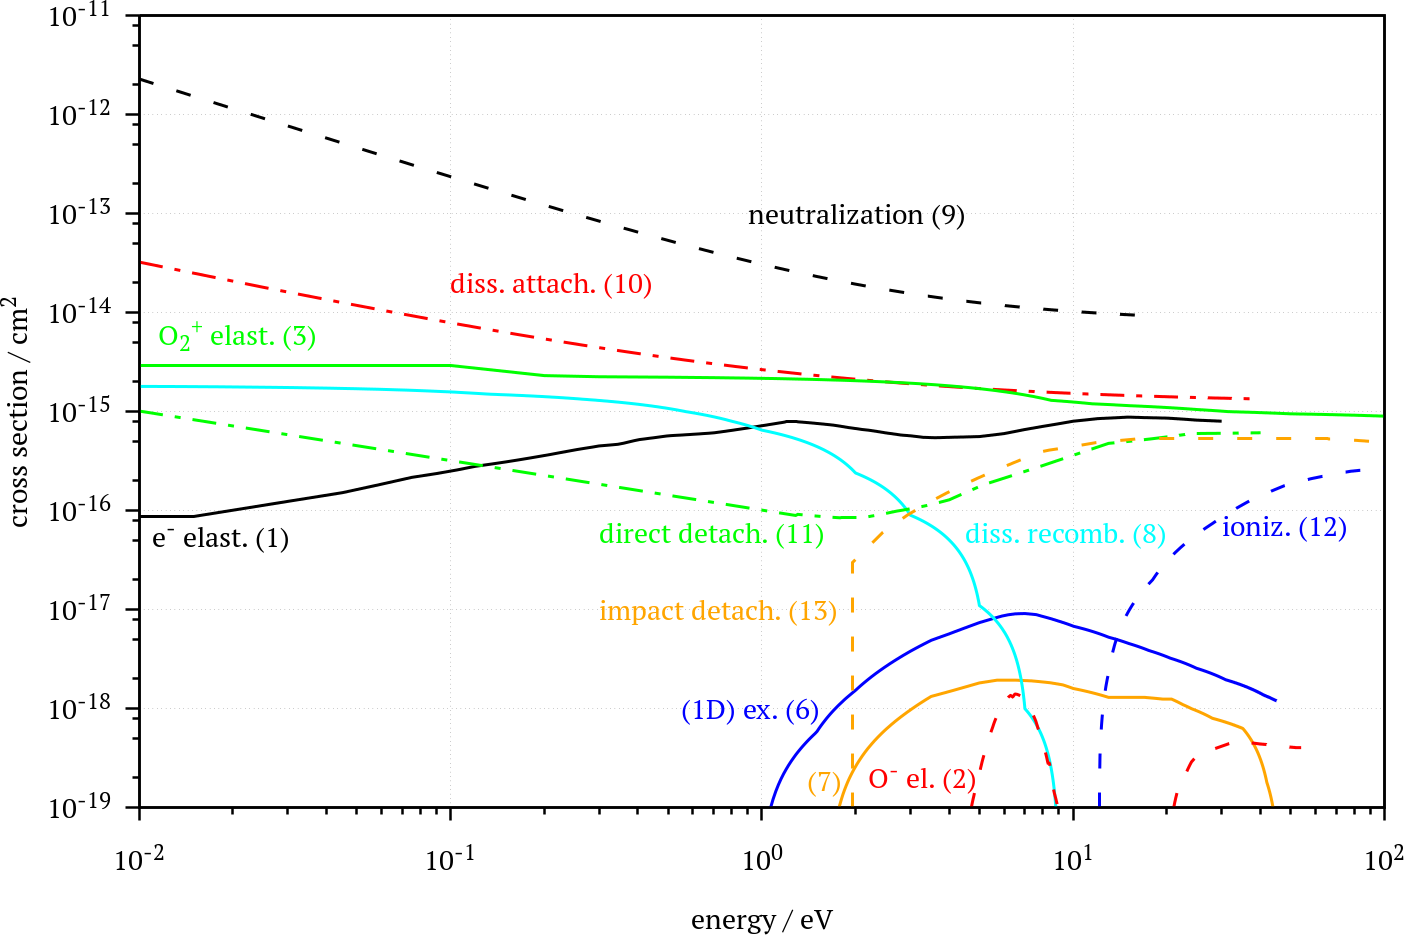
\includegraphics[width=1.0\textwidth]{figures/xsections.png}
				\caption{%
				Cross section data of electron energy loss, electron and ion production/loss and elastic scattering collisions from~\cite{Gudmundsson13} and~\cite{Bronold07b}. The corresponding reaction equations are shown in~\autoref{tab:cross_sections}.}%
				\label{fig:cross_sections}	
			\end{figure}	
